\documentclass[1p]{elsarticle_modified}
%\bibliographystyle{elsarticle-num}

%\usepackage[colorlinks]{hyperref}
%\usepackage{abbrmath_seonhwa} %\Abb, \Ascr, \Acal ,\Abf, \Afrak
\usepackage{amsfonts}
\usepackage{amssymb}
\usepackage{amsmath}
\usepackage{amsthm}
\usepackage{scalefnt}
\usepackage{amsbsy}
\usepackage{kotex}
\usepackage{caption}
\usepackage{subfig}
\usepackage{color}
\usepackage{graphicx}
\usepackage{xcolor} %% white, black, red, green, blue, cyan, magenta, yellow
\usepackage{float}
\usepackage{setspace}
\usepackage{hyperref}

\usepackage{tikz}
\usetikzlibrary{arrows}

\usepackage{multirow}
\usepackage{array} % fixed length table
\usepackage{hhline}

%%%%%%%%%%%%%%%%%%%%%
\makeatletter
\renewcommand*\env@matrix[1][\arraystretch]{%
	\edef\arraystretch{#1}%
	\hskip -\arraycolsep
	\let\@ifnextchar\new@ifnextchar
	\array{*\c@MaxMatrixCols c}}
\makeatother %https://tex.stackexchange.com/questions/14071/how-can-i-increase-the-line-spacing-in-a-matrix
%%%%%%%%%%%%%%%

\usepackage[normalem]{ulem}

\newcommand{\msout}[1]{\ifmmode\text{\sout{\ensuremath{#1}}}\else\sout{#1}\fi}
%SOURCE: \msout is \stkout macro in https://tex.stackexchange.com/questions/20609/strikeout-in-math-mode

\newcommand{\cancel}[1]{
	\ifmmode
	{\color{red}\msout{#1}}
	\else
	{\color{red}\sout{#1}}
	\fi
}

\newcommand{\add}[1]{
	{\color{blue}\uwave{#1}}
}

\newcommand{\replace}[2]{
	\ifmmode
	{\color{red}\msout{#1}}{\color{blue}\uwave{#2}}
	\else
	{\color{red}\sout{#1}}{\color{blue}\uwave{#2}}
	\fi
}

\newcommand{\Sol}{\mathcal{S}} %segment
\newcommand{\D}{D} %diagram
\newcommand{\A}{\mathcal{A}} %arc


%%%%%%%%%%%%%%%%%%%%%%%%%%%%%5 test

\def\sl{\operatorname{\textup{SL}}(2,\Cbb)}
\def\psl{\operatorname{\textup{PSL}}(2,\Cbb)}
\def\quan{\mkern 1mu \triangleright \mkern 1mu}

\theoremstyle{definition}
\newtheorem{thm}{Theorem}[section]
\newtheorem{prop}[thm]{Proposition}
\newtheorem{lem}[thm]{Lemma}
\newtheorem{ques}[thm]{Question}
\newtheorem{cor}[thm]{Corollary}
\newtheorem{defn}[thm]{Definition}
\newtheorem{exam}[thm]{Example}
\newtheorem{rmk}[thm]{Remark}
\newtheorem{alg}[thm]{Algorithm}

\newcommand{\I}{\sqrt{-1}}
\begin{document}

%\begin{frontmatter}
%
%\title{Boundary parabolic representations of knots up to 8 crossings}
%
%%% Group authors per affiliation:
%\author{Yunhi Cho} 
%\address{Department of Mathematics, University of Seoul, Seoul, Korea}
%\ead{yhcho@uos.ac.kr}
%
%
%\author{Seonhwa Kim} %\fnref{s_kim}}
%\address{Center for Geometry and Physics, Institute for Basic Science, Pohang, 37673, Korea}
%\ead{ryeona17@ibs.re.kr}
%
%\author{Hyuk Kim}
%\address{Department of Mathematical Sciences, Seoul National University, Seoul 08826, Korea}
%\ead{hyukkim@snu.ac.kr}
%
%\author{Seokbeom Yoon}
%\address{Department of Mathematical Sciences, Seoul National University, Seoul, 08826,  Korea}
%\ead{sbyoon15@snu.ac.kr}
%
%\begin{abstract}
%We find all boundary parabolic representation of knots up to 8 crossings.
%
%\end{abstract}
%\begin{keyword}
%    \MSC[2010] 57M25 
%\end{keyword}
%
%\end{frontmatter}

%\linenumbers
%\tableofcontents
%
\newcommand\colored[1]{\textcolor{white}{\rule[-0.35ex]{0.8em}{1.4ex}}\kern-0.8em\color{red} #1}%
%\newcommand\colored[1]{\textcolor{white}{ #1}\kern-2.17ex	\textcolor{white}{ #1}\kern-1.81ex	\textcolor{white}{ #1}\kern-2.15ex\color{red}#1	}

{\Large $\underline{12n_{0885}~(K12n_{0885})}$}

\setlength{\tabcolsep}{10pt}
\renewcommand{\arraystretch}{1.6}
\vspace{1cm}\begin{tabular}{m{100pt}>{\centering\arraybackslash}m{274pt}}
\multirow{5}{120pt}{
	\centering
	\includegraphics[width=112pt]{../../../GIT/diagram.site/Diagrams/png/2974_12n_0885.png}\\
\ \ \ A knot diagram\footnotemark}&
\allowdisplaybreaks
\textbf{Linearized knot diagam} \\
\cline{2-2}
 &
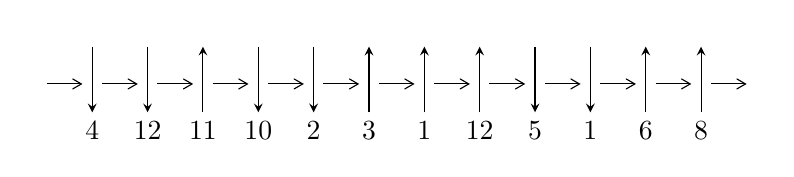
\begin{tikzpicture}[x=20pt, y=17pt]
	% nodes
	\node (C0) at (0, 0) {};
	\node (C1) at (1, 0) {};
	\node (C1U) at (1, +1) {};
	\node (C1D) at (1, -1) {4};

	\node (C2) at (2, 0) {};
	\node (C2U) at (2, +1) {};
	\node (C2D) at (2, -1) {12};

	\node (C3) at (3, 0) {};
	\node (C3U) at (3, +1) {};
	\node (C3D) at (3, -1) {11};

	\node (C4) at (4, 0) {};
	\node (C4U) at (4, +1) {};
	\node (C4D) at (4, -1) {10};

	\node (C5) at (5, 0) {};
	\node (C5U) at (5, +1) {};
	\node (C5D) at (5, -1) {2};

	\node (C6) at (6, 0) {};
	\node (C6U) at (6, +1) {};
	\node (C6D) at (6, -1) {3};

	\node (C7) at (7, 0) {};
	\node (C7U) at (7, +1) {};
	\node (C7D) at (7, -1) {1};

	\node (C8) at (8, 0) {};
	\node (C8U) at (8, +1) {};
	\node (C8D) at (8, -1) {12};

	\node (C9) at (9, 0) {};
	\node (C9U) at (9, +1) {};
	\node (C9D) at (9, -1) {5};

	\node (C10) at (10, 0) {};
	\node (C10U) at (10, +1) {};
	\node (C10D) at (10, -1) {1};

	\node (C11) at (11, 0) {};
	\node (C11U) at (11, +1) {};
	\node (C11D) at (11, -1) {6};

	\node (C12) at (12, 0) {};
	\node (C12U) at (12, +1) {};
	\node (C12D) at (12, -1) {8};
	\node (C13) at (13, 0) {};

	% arrows
	\draw[->,>={angle 60}]
	(C0) edge (C1) (C1) edge (C2) (C2) edge (C3) (C3) edge (C4) (C4) edge (C5) (C5) edge (C6) (C6) edge (C7) (C7) edge (C8) (C8) edge (C9) (C9) edge (C10) (C10) edge (C11) (C11) edge (C12) (C12) edge (C13) ;	\draw[->,>=stealth]
	(C1U) edge (C1D) (C2U) edge (C2D) (C3D) edge (C3U) (C4U) edge (C4D) (C5U) edge (C5D) (C6D) edge (C6U) (C7D) edge (C7U) (C8D) edge (C8U) (C9U) edge (C9D) (C10U) edge (C10D) (C11D) edge (C11U) (C12D) edge (C12U) ;
	\end{tikzpicture} \\
\hhline{~~} \\& 
\textbf{Solving Sequence} \\ \cline{2-2} 
 &
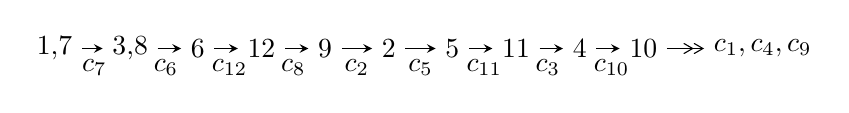
\begin{tikzpicture}[x=23pt, y=7pt]
	% node
	\node (A0) at (-1/8, 0) {1,7};
	\node (A1) at (17/16, 0) {3,8};
	\node (A2) at (17/8, 0) {6};
	\node (A3) at (25/8, 0) {12};
	\node (A4) at (33/8, 0) {9};
	\node (A5) at (41/8, 0) {2};
	\node (A6) at (49/8, 0) {5};
	\node (A7) at (57/8, 0) {11};
	\node (A8) at (65/8, 0) {4};
	\node (A9) at (73/8, 0) {10};
	\node (C1) at (1/2, -1) {$c_{7}$};
	\node (C2) at (13/8, -1) {$c_{6}$};
	\node (C3) at (21/8, -1) {$c_{12}$};
	\node (C4) at (29/8, -1) {$c_{8}$};
	\node (C5) at (37/8, -1) {$c_{2}$};
	\node (C6) at (45/8, -1) {$c_{5}$};
	\node (C7) at (53/8, -1) {$c_{11}$};
	\node (C8) at (61/8, -1) {$c_{3}$};
	\node (C9) at (69/8, -1) {$c_{10}$};
	\node (A10) at (11, 0) {$c_{1},c_{4},c_{9}$};

	% edge
	\draw[->,>=stealth]	
	(A0) edge (A1) (A1) edge (A2) (A2) edge (A3) (A3) edge (A4) (A4) edge (A5) (A5) edge (A6) (A6) edge (A7) (A7) edge (A8) (A8) edge (A9) ;
	\draw[->>,>={angle 60}]	
	(A9) edge (A10);
\end{tikzpicture} \\ 

\end{tabular} \\

\footnotetext{
The image of knot diagram is generated by the software ``\textbf{Draw programme}" developed by Andrew Bartholomew(\url{http://www.layer8.co.uk/maths/draw/index.htm\#Running-draw}), where we modified some parts for our purpose(\url{https://github.com/CATsTAILs/LinksPainter}).
}\phantom \\ \newline 
\centering \textbf{Ideals for irreducible components\footnotemark of $X_{\text{par}}$} 
 
\begin{align*}
I^u_{1}&=\langle 
-7.56659\times10^{393} u^{111}+5.31853\times10^{393} u^{110}+\cdots+6.91031\times10^{394} b+9.38589\times10^{396},\\
\phantom{I^u_{1}}&\phantom{= \langle  }5.28363\times10^{395} u^{111}-1.20999\times10^{395} u^{110}+\cdots+1.17475\times10^{396} a-6.03150\times10^{398},\\
\phantom{I^u_{1}}&\phantom{= \langle  }u^{112}+2 u^{111}+\cdots+459 u+289\rangle \\
I^u_{2}&=\langle 
2210073442011996 u^{37}+2571675910997884 u^{36}+\cdots+123978150535333 b+4009129869435240,\\
\phantom{I^u_{2}}&\phantom{= \langle  }-5.10927\times10^{15} u^{37}-2.87486\times10^{15} u^{36}+\cdots+1.23978\times10^{14} a-2.73599\times10^{15},\;u^{38}+u^{37}+\cdots+8 u+1\rangle \\
\\
\end{align*}
\raggedright * 2 irreducible components of $\dim_{\mathbb{C}}=0$, with total 150 representations.\\
\footnotetext{All coefficients of polynomials are rational numbers. But the coefficients are sometimes approximated in decimal forms when there is not enough margin.}
\newpage
\renewcommand{\arraystretch}{1}
\centering \section*{I. $I^u_{1}= \langle -7.57\times10^{393} u^{111}+5.32\times10^{393} u^{110}+\cdots+6.91\times10^{394} b+9.39\times10^{396},\;5.28\times10^{395} u^{111}-1.21\times10^{395} u^{110}+\cdots+1.17\times10^{396} a-6.03\times10^{398},\;u^{112}+2 u^{111}+\cdots+459 u+289 \rangle$}
\flushleft \textbf{(i) Arc colorings}\\
\begin{tabular}{m{7pt} m{180pt} m{7pt} m{180pt} }
\flushright $a_{1}=$&$\begin{pmatrix}0\\u\end{pmatrix}$ \\
\flushright $a_{7}=$&$\begin{pmatrix}1\\0\end{pmatrix}$ \\
\flushright $a_{3}=$&$\begin{pmatrix}-0.449765 u^{111}+0.103000 u^{110}+\cdots+624.384 u+513.428\\0.109497 u^{111}-0.0769651 u^{110}+\cdots-103.765 u-135.824\end{pmatrix}$ \\
\flushright $a_{8}=$&$\begin{pmatrix}1\\- u^2\end{pmatrix}$ \\
\flushright $a_{6}=$&$\begin{pmatrix}1.62871 u^{111}+2.34289 u^{110}+\cdots-75.5842 u-639.880\\-0.509787 u^{111}-1.11956 u^{110}+\cdots-328.017 u-70.2302\end{pmatrix}$ \\
\flushright $a_{12}=$&$\begin{pmatrix}- u\\u^3+u\end{pmatrix}$ \\
\flushright $a_{9}=$&$\begin{pmatrix}u^2+1\\- u^4-2 u^2\end{pmatrix}$ \\
\flushright $a_{2}=$&$\begin{pmatrix}-0.386026 u^{111}+0.114229 u^{110}+\cdots+604.557 u+480.705\\0.0590533 u^{111}-0.163272 u^{110}+\cdots-118.876 u-136.698\end{pmatrix}$ \\
\flushright $a_{5}=$&$\begin{pmatrix}2.32825 u^{111}+5.23070 u^{110}+\cdots+2599.85 u+493.752\\2.02780 u^{111}+3.98309 u^{110}+\cdots+1426.33 u-5.42016\end{pmatrix}$ \\
\flushright $a_{11}=$&$\begin{pmatrix}1.31050 u^{111}+1.18092 u^{110}+\cdots-634.760 u-1006.77\\-0.942003 u^{111}-2.32694 u^{110}+\cdots-1021.96 u-273.577\end{pmatrix}$ \\
\flushright $a_{4}=$&$\begin{pmatrix}-0.204868 u^{111}-0.104364 u^{110}+\cdots-296.422 u+33.2570\\-0.836701 u^{111}-2.01743 u^{110}+\cdots-1104.03 u-284.727\end{pmatrix}$ \\
\flushright $a_{10}=$&$\begin{pmatrix}1.31050 u^{111}+1.18092 u^{110}+\cdots-634.760 u-1006.77\\-0.361452 u^{111}-1.80415 u^{110}+\cdots-1304.23 u-689.763\end{pmatrix}$\\&\end{tabular}
\flushleft \textbf{(ii) Obstruction class $= -1$}\\~\\
\flushleft \textbf{(iii) Cusp Shapes $= 4.15892 u^{111}+12.5312 u^{110}+\cdots+6892.43 u+2672.74$}\\~\\
\newpage\renewcommand{\arraystretch}{1}
\flushleft \textbf{(iv) u-Polynomials at the component}\newline \\
\begin{tabular}{m{50pt}|m{274pt}}
Crossings & \hspace{64pt}u-Polynomials at each crossing \\
\hline $$\begin{aligned}c_{1}\end{aligned}$$&$\begin{aligned}
&u^{112}+11 u^{111}+\cdots-11 u+1
\end{aligned}$\\
\hline $$\begin{aligned}c_{2}\end{aligned}$$&$\begin{aligned}
&u^{112}+2 u^{111}+\cdots-245060 u+69175
\end{aligned}$\\
\hline $$\begin{aligned}c_{3}\end{aligned}$$&$\begin{aligned}
&u^{112}+3 u^{111}+\cdots+3092 u+3329
\end{aligned}$\\
\hline $$\begin{aligned}c_{4},c_{9}\end{aligned}$$&$\begin{aligned}
&u^{112}+u^{111}+\cdots+193 u+1
\end{aligned}$\\
\hline $$\begin{aligned}c_{5}\end{aligned}$$&$\begin{aligned}
&u^{112}-2 u^{111}+\cdots-1572680 u+716581
\end{aligned}$\\
\hline $$\begin{aligned}c_{6}\end{aligned}$$&$\begin{aligned}
&u^{112}-7 u^{111}+\cdots+312132 u+23423
\end{aligned}$\\
\hline $$\begin{aligned}c_{7},c_{8},c_{12}\end{aligned}$$&$\begin{aligned}
&u^{112}-2 u^{111}+\cdots-459 u+289
\end{aligned}$\\
\hline $$\begin{aligned}c_{10}\end{aligned}$$&$\begin{aligned}
&u^{112}+u^{111}+\cdots+72748 u+7829
\end{aligned}$\\
\hline $$\begin{aligned}c_{11}\end{aligned}$$&$\begin{aligned}
&u^{112}-2 u^{111}+\cdots+16 u+1
\end{aligned}$\\
\hline
\end{tabular}\\~\\
\newpage\renewcommand{\arraystretch}{1}
\flushleft \textbf{(v) Riley Polynomials at the component}\newline \\
\begin{tabular}{m{50pt}|m{274pt}}
Crossings & \hspace{64pt}Riley Polynomials at each crossing \\
\hline $$\begin{aligned}c_{1}\end{aligned}$$&$\begin{aligned}
&y^{112}-15 y^{111}+\cdots-37 y+1
\end{aligned}$\\
\hline $$\begin{aligned}c_{2}\end{aligned}$$&$\begin{aligned}
&y^{112}+20 y^{111}+\cdots+765903812450 y+4785180625
\end{aligned}$\\
\hline $$\begin{aligned}c_{3}\end{aligned}$$&$\begin{aligned}
&y^{112}+17 y^{111}+\cdots-245986044 y+11082241
\end{aligned}$\\
\hline $$\begin{aligned}c_{4},c_{9}\end{aligned}$$&$\begin{aligned}
&y^{112}+97 y^{111}+\cdots+33271 y+1
\end{aligned}$\\
\hline $$\begin{aligned}c_{5}\end{aligned}$$&$\begin{aligned}
&y^{112}+18 y^{111}+\cdots-11466541483818 y+513488329561
\end{aligned}$\\
\hline $$\begin{aligned}c_{6}\end{aligned}$$&$\begin{aligned}
&y^{112}-9 y^{111}+\cdots-1897506918 y+548636929
\end{aligned}$\\
\hline $$\begin{aligned}c_{7},c_{8},c_{12}\end{aligned}$$&$\begin{aligned}
&y^{112}+48 y^{111}+\cdots+4810983 y+83521
\end{aligned}$\\
\hline $$\begin{aligned}c_{10}\end{aligned}$$&$\begin{aligned}
&y^{112}+39 y^{111}+\cdots-3571112828 y+61293241
\end{aligned}$\\
\hline $$\begin{aligned}c_{11}\end{aligned}$$&$\begin{aligned}
&y^{112}+30 y^{111}+\cdots+192 y+1
\end{aligned}$\\
\hline
\end{tabular}\\~\\
\newpage\flushleft \textbf{(vi) Complex Volumes and Cusp Shapes}
$$\begin{array}{c|c|c}  
\text{Solutions to }I^u_{1}& \I (\text{vol} + \sqrt{-1}CS) & \text{Cusp shape}\\
 \hline 
\begin{aligned}
u &= \phantom{-}0.010224 + 1.010630 I \\
a &= -0.565108 + 1.075190 I \\
b &= -0.481314 + 1.126550 I\end{aligned}
 & -2.39260 - 3.77429 I & \phantom{-0.000000 } 0 \\ \hline\begin{aligned}
u &= \phantom{-}0.010224 - 1.010630 I \\
a &= -0.565108 - 1.075190 I \\
b &= -0.481314 - 1.126550 I\end{aligned}
 & -2.39260 + 3.77429 I & \phantom{-0.000000 } 0 \\ \hline\begin{aligned}
u &= -0.812945 + 0.629113 I \\
a &= \phantom{-}1.006710 - 0.116134 I \\
b &= -1.064790 + 0.062857 I\end{aligned}
 & \phantom{-}2.85892 - 1.65749 I & \phantom{-0.000000 } 0 \\ \hline\begin{aligned}
u &= -0.812945 - 0.629113 I \\
a &= \phantom{-}1.006710 + 0.116134 I \\
b &= -1.064790 - 0.062857 I\end{aligned}
 & \phantom{-}2.85892 + 1.65749 I & \phantom{-0.000000 } 0 \\ \hline\begin{aligned}
u &= \phantom{-}0.717527 + 0.651268 I \\
a &= \phantom{-}0.88811 - 1.11391 I \\
b &= -1.20948 + 0.76438 I\end{aligned}
 & \phantom{-}2.60302 - 1.92558 I & \phantom{-0.000000 } 0 \\ \hline\begin{aligned}
u &= \phantom{-}0.717527 - 0.651268 I \\
a &= \phantom{-}0.88811 + 1.11391 I \\
b &= -1.20948 - 0.76438 I\end{aligned}
 & \phantom{-}2.60302 + 1.92558 I & \phantom{-0.000000 } 0 \\ \hline\begin{aligned}
u &= -0.593598 + 0.753642 I \\
a &= -0.688837 + 0.229659 I \\
b &= \phantom{-}0.628603 + 0.743308 I\end{aligned}
 & -0.256622 - 0.586000 I & \phantom{-0.000000 } 0 \\ \hline\begin{aligned}
u &= -0.593598 - 0.753642 I \\
a &= -0.688837 - 0.229659 I \\
b &= \phantom{-}0.628603 - 0.743308 I\end{aligned}
 & -0.256622 + 0.586000 I & \phantom{-0.000000 } 0 \\ \hline\begin{aligned}
u &= -0.605633 + 0.863987 I \\
a &= -1.14259 - 1.39421 I \\
b &= \phantom{-}0.441758 - 0.712141 I\end{aligned}
 & -0.56474 - 4.14412 I & \phantom{-0.000000 } 0 \\ \hline\begin{aligned}
u &= -0.605633 - 0.863987 I \\
a &= -1.14259 + 1.39421 I \\
b &= \phantom{-}0.441758 + 0.712141 I\end{aligned}
 & -0.56474 + 4.14412 I & \phantom{-0.000000 } 0\\
 \hline 
 \end{array}$$\newpage$$\begin{array}{c|c|c}  
\text{Solutions to }I^u_{1}& \I (\text{vol} + \sqrt{-1}CS) & \text{Cusp shape}\\
 \hline 
\begin{aligned}
u &= -0.600038 + 0.889896 I \\
a &= -1.318550 - 0.259925 I \\
b &= \phantom{-}0.324086 - 0.261126 I\end{aligned}
 & \phantom{-}0.08866 - 2.33112 I & \phantom{-0.000000 } 0 \\ \hline\begin{aligned}
u &= -0.600038 - 0.889896 I \\
a &= -1.318550 + 0.259925 I \\
b &= \phantom{-}0.324086 + 0.261126 I\end{aligned}
 & \phantom{-}0.08866 + 2.33112 I & \phantom{-0.000000 } 0 \\ \hline\begin{aligned}
u &= -0.128704 + 0.916543 I \\
a &= -1.10668 - 1.46919 I \\
b &= \phantom{-}0.646085 - 0.883968 I\end{aligned}
 & \phantom{-}0.81583 - 5.97740 I & \phantom{-0.000000 } 0 \\ \hline\begin{aligned}
u &= -0.128704 - 0.916543 I \\
a &= -1.10668 + 1.46919 I \\
b &= \phantom{-}0.646085 + 0.883968 I\end{aligned}
 & \phantom{-}0.81583 + 5.97740 I & \phantom{-0.000000 } 0 \\ \hline\begin{aligned}
u &= \phantom{-}0.707129 + 0.817332 I \\
a &= \phantom{-}0.518561 - 0.874958 I \\
b &= -0.627852 + 0.677662 I\end{aligned}
 & \phantom{-}2.12801 - 3.19948 I & \phantom{-0.000000 } 0 \\ \hline\begin{aligned}
u &= \phantom{-}0.707129 - 0.817332 I \\
a &= \phantom{-}0.518561 + 0.874958 I \\
b &= -0.627852 - 0.677662 I\end{aligned}
 & \phantom{-}2.12801 + 3.19948 I & \phantom{-0.000000 } 0 \\ \hline\begin{aligned}
u &= \phantom{-}0.703734 + 0.941380 I \\
a &= \phantom{-}1.77010 - 0.29305 I \\
b &= -0.822358 - 1.043520 I\end{aligned}
 & \phantom{-}1.71948 + 8.64037 I & \phantom{-0.000000 } 0 \\ \hline\begin{aligned}
u &= \phantom{-}0.703734 - 0.941380 I \\
a &= \phantom{-}1.77010 + 0.29305 I \\
b &= -0.822358 + 1.043520 I\end{aligned}
 & \phantom{-}1.71948 - 8.64037 I & \phantom{-0.000000 } 0 \\ \hline\begin{aligned}
u &= -0.772980 + 0.886031 I \\
a &= -0.641107 - 0.533275 I \\
b &= \phantom{-}0.670222 + 0.169400 I\end{aligned}
 & \phantom{-}0.44460 - 1.60261 I & \phantom{-0.000000 } 0 \\ \hline\begin{aligned}
u &= -0.772980 - 0.886031 I \\
a &= -0.641107 + 0.533275 I \\
b &= \phantom{-}0.670222 - 0.169400 I\end{aligned}
 & \phantom{-}0.44460 + 1.60261 I & \phantom{-0.000000 } 0\\
 \hline 
 \end{array}$$\newpage$$\begin{array}{c|c|c}  
\text{Solutions to }I^u_{1}& \I (\text{vol} + \sqrt{-1}CS) & \text{Cusp shape}\\
 \hline 
\begin{aligned}
u &= -0.840246 + 0.831516 I \\
a &= -1.228540 - 0.073457 I \\
b &= \phantom{-}0.894973 - 0.595162 I\end{aligned}
 & \phantom{-}0.66730 - 4.44117 I & \phantom{-0.000000 } 0 \\ \hline\begin{aligned}
u &= -0.840246 - 0.831516 I \\
a &= -1.228540 + 0.073457 I \\
b &= \phantom{-}0.894973 + 0.595162 I\end{aligned}
 & \phantom{-}0.66730 + 4.44117 I & \phantom{-0.000000 } 0 \\ \hline\begin{aligned}
u &= -0.840144 + 0.842227 I \\
a &= -1.65760 - 0.34454 I \\
b &= \phantom{-}1.48014 - 1.50201 I\end{aligned}
 & \phantom{-}6.16132 - 7.16661 I & \phantom{-0.000000 } 0 \\ \hline\begin{aligned}
u &= -0.840144 - 0.842227 I \\
a &= -1.65760 + 0.34454 I \\
b &= \phantom{-}1.48014 + 1.50201 I\end{aligned}
 & \phantom{-}6.16132 + 7.16661 I & \phantom{-0.000000 } 0 \\ \hline\begin{aligned}
u &= \phantom{-}0.954188 + 0.714485 I \\
a &= -0.800464 + 0.829167 I \\
b &= \phantom{-}1.321720 - 0.471927 I\end{aligned}
 & \phantom{-}1.17560 - 5.72024 I & \phantom{-0.000000 } 0 \\ \hline\begin{aligned}
u &= \phantom{-}0.954188 - 0.714485 I \\
a &= -0.800464 - 0.829167 I \\
b &= \phantom{-}1.321720 + 0.471927 I\end{aligned}
 & \phantom{-}1.17560 + 5.72024 I & \phantom{-0.000000 } 0 \\ \hline\begin{aligned}
u &= -0.059036 + 0.804581 I \\
a &= -3.99094 - 0.63958 I \\
b &= -0.255241 - 0.160120 I\end{aligned}
 & -2.07878 - 6.23665 I & \phantom{-0.000000 } 0 \\ \hline\begin{aligned}
u &= -0.059036 - 0.804581 I \\
a &= -3.99094 + 0.63958 I \\
b &= -0.255241 + 0.160120 I\end{aligned}
 & -2.07878 + 6.23665 I & \phantom{-0.000000 } 0 \\ \hline\begin{aligned}
u &= \phantom{-}0.089804 + 0.797050 I \\
a &= -0.999786 + 0.239726 I \\
b &= -0.245820 + 1.058670 I\end{aligned}
 & -1.51333 - 1.66775 I & \phantom{-0.000000 } 0 \\ \hline\begin{aligned}
u &= \phantom{-}0.089804 - 0.797050 I \\
a &= -0.999786 - 0.239726 I \\
b &= -0.245820 - 1.058670 I\end{aligned}
 & -1.51333 + 1.66775 I & \phantom{-0.000000 } 0\\
 \hline 
 \end{array}$$\newpage$$\begin{array}{c|c|c}  
\text{Solutions to }I^u_{1}& \I (\text{vol} + \sqrt{-1}CS) & \text{Cusp shape}\\
 \hline 
\begin{aligned}
u &= -0.448545 + 0.662618 I \\
a &= -0.546947 + 0.089449 I \\
b &= \phantom{-}0.086739 + 0.262305 I\end{aligned}
 & \phantom{-}0.04786 - 1.76911 I & \phantom{-0.000000 } 0 \\ \hline\begin{aligned}
u &= -0.448545 - 0.662618 I \\
a &= -0.546947 - 0.089449 I \\
b &= \phantom{-}0.086739 - 0.262305 I\end{aligned}
 & \phantom{-}0.04786 + 1.76911 I & \phantom{-0.000000 } 0 \\ \hline\begin{aligned}
u &= \phantom{-}1.101710 + 0.476207 I \\
a &= -0.808553 + 0.079696 I \\
b &= \phantom{-}1.091240 - 0.186893 I\end{aligned}
 & \phantom{-}8.51602 - 4.13389 I & \phantom{-0.000000 } 0 \\ \hline\begin{aligned}
u &= \phantom{-}1.101710 - 0.476207 I \\
a &= -0.808553 - 0.079696 I \\
b &= \phantom{-}1.091240 + 0.186893 I\end{aligned}
 & \phantom{-}8.51602 + 4.13389 I & \phantom{-0.000000 } 0 \\ \hline\begin{aligned}
u &= \phantom{-}0.851258 + 0.850692 I \\
a &= \phantom{-}0.766990 - 0.907488 I \\
b &= -0.295633 - 1.125820 I\end{aligned}
 & \phantom{-}2.71011 + 8.27807 I & \phantom{-0.000000 } 0 \\ \hline\begin{aligned}
u &= \phantom{-}0.851258 - 0.850692 I \\
a &= \phantom{-}0.766990 + 0.907488 I \\
b &= -0.295633 + 1.125820 I\end{aligned}
 & \phantom{-}2.71011 - 8.27807 I & \phantom{-0.000000 } 0 \\ \hline\begin{aligned}
u &= \phantom{-}0.353295 + 0.703837 I \\
a &= \phantom{-}0.428741 + 0.636394 I \\
b &= \phantom{-}0.36891 - 1.66008 I\end{aligned}
 & -2.96846 + 3.39223 I & \phantom{-0.000000 } 0 \\ \hline\begin{aligned}
u &= \phantom{-}0.353295 - 0.703837 I \\
a &= \phantom{-}0.428741 - 0.636394 I \\
b &= \phantom{-}0.36891 + 1.66008 I\end{aligned}
 & -2.96846 - 3.39223 I & \phantom{-0.000000 } 0 \\ \hline\begin{aligned}
u &= -0.885092 + 0.845173 I \\
a &= -0.552187 + 0.806856 I \\
b &= -1.00714 - 2.45174 I\end{aligned}
 & \phantom{-}3.48223 - 7.89026 I & \phantom{-0.000000 } 0 \\ \hline\begin{aligned}
u &= -0.885092 - 0.845173 I \\
a &= -0.552187 - 0.806856 I \\
b &= -1.00714 + 2.45174 I\end{aligned}
 & \phantom{-}3.48223 + 7.89026 I & \phantom{-0.000000 } 0\\
 \hline 
 \end{array}$$\newpage$$\begin{array}{c|c|c}  
\text{Solutions to }I^u_{1}& \I (\text{vol} + \sqrt{-1}CS) & \text{Cusp shape}\\
 \hline 
\begin{aligned}
u &= -1.168000 + 0.425870 I \\
a &= -0.974961 - 0.465503 I \\
b &= \phantom{-}1.39657 + 0.95645 I\end{aligned}
 & \phantom{-}7.99615 + 2.91423 I & \phantom{-0.000000 } 0 \\ \hline\begin{aligned}
u &= -1.168000 - 0.425870 I \\
a &= -0.974961 + 0.465503 I \\
b &= \phantom{-}1.39657 - 0.95645 I\end{aligned}
 & \phantom{-}7.99615 - 2.91423 I & \phantom{-0.000000 } 0 \\ \hline\begin{aligned}
u &= \phantom{-}0.153101 + 0.737841 I \\
a &= \phantom{-}3.02088 - 0.15622 I \\
b &= -1.64182 - 0.30778 I\end{aligned}
 & -1.82730 + 6.62412 I & \phantom{-0.000000 } 0 \\ \hline\begin{aligned}
u &= \phantom{-}0.153101 - 0.737841 I \\
a &= \phantom{-}3.02088 + 0.15622 I \\
b &= -1.64182 + 0.30778 I\end{aligned}
 & -1.82730 - 6.62412 I & \phantom{-0.000000 } 0 \\ \hline\begin{aligned}
u &= -0.112644 + 1.241550 I \\
a &= \phantom{-}0.153891 + 0.235932 I \\
b &= \phantom{-}0.778653 + 0.677481 I\end{aligned}
 & \phantom{-}1.42418 - 1.09821 I & \phantom{-0.000000 } 0 \\ \hline\begin{aligned}
u &= -0.112644 - 1.241550 I \\
a &= \phantom{-}0.153891 - 0.235932 I \\
b &= \phantom{-}0.778653 - 0.677481 I\end{aligned}
 & \phantom{-}1.42418 + 1.09821 I & \phantom{-0.000000 } 0 \\ \hline\begin{aligned}
u &= \phantom{-}0.864442 + 0.899652 I \\
a &= \phantom{-}1.182090 - 0.278870 I \\
b &= -0.572044 - 0.187611 I\end{aligned}
 & \phantom{-}2.09442 + 3.19547 I & \phantom{-0.000000 } 0 \\ \hline\begin{aligned}
u &= \phantom{-}0.864442 - 0.899652 I \\
a &= \phantom{-}1.182090 + 0.278870 I \\
b &= -0.572044 + 0.187611 I\end{aligned}
 & \phantom{-}2.09442 - 3.19547 I & \phantom{-0.000000 } 0 \\ \hline\begin{aligned}
u &= \phantom{-}0.669954 + 1.054250 I \\
a &= \phantom{-}1.63340 - 0.76545 I \\
b &= -1.23338 - 1.10889 I\end{aligned}
 & \phantom{-}1.37396 + 7.30647 I & \phantom{-0.000000 } 0 \\ \hline\begin{aligned}
u &= \phantom{-}0.669954 - 1.054250 I \\
a &= \phantom{-}1.63340 + 0.76545 I \\
b &= -1.23338 + 1.10889 I\end{aligned}
 & \phantom{-}1.37396 - 7.30647 I & \phantom{-0.000000 } 0\\
 \hline 
 \end{array}$$\newpage$$\begin{array}{c|c|c}  
\text{Solutions to }I^u_{1}& \I (\text{vol} + \sqrt{-1}CS) & \text{Cusp shape}\\
 \hline 
\begin{aligned}
u &= \phantom{-}0.843299 + 0.923345 I \\
a &= -1.270000 + 0.184509 I \\
b &= \phantom{-}1.021560 + 0.207033 I\end{aligned}
 & \phantom{-}6.94915 + 8.95337 I & \phantom{-0.000000 } 0 \\ \hline\begin{aligned}
u &= \phantom{-}0.843299 - 0.923345 I \\
a &= -1.270000 - 0.184509 I \\
b &= \phantom{-}1.021560 - 0.207033 I\end{aligned}
 & \phantom{-}6.94915 - 8.95337 I & \phantom{-0.000000 } 0 \\ \hline\begin{aligned}
u &= -0.034984 + 0.747340 I \\
a &= -0.49181 + 2.26827 I \\
b &= -0.023193 + 0.891633 I\end{aligned}
 & -2.96917 - 1.87590 I & \phantom{-0.000000 } 0 \\ \hline\begin{aligned}
u &= -0.034984 - 0.747340 I \\
a &= -0.49181 - 2.26827 I \\
b &= -0.023193 - 0.891633 I\end{aligned}
 & -2.96917 + 1.87590 I & \phantom{-0.000000 } 0 \\ \hline\begin{aligned}
u &= \phantom{-}0.862675 + 0.908381 I \\
a &= \phantom{-}1.19647 - 0.84731 I \\
b &= -1.80368 - 0.35487 I\end{aligned}
 & \phantom{-}6.71889 + 3.19714 I & \phantom{-0.000000 } 0 \\ \hline\begin{aligned}
u &= \phantom{-}0.862675 - 0.908381 I \\
a &= \phantom{-}1.19647 + 0.84731 I \\
b &= -1.80368 + 0.35487 I\end{aligned}
 & \phantom{-}6.71889 - 3.19714 I & \phantom{-0.000000 } 0 \\ \hline\begin{aligned}
u &= \phantom{-}0.867416 + 0.906743 I \\
a &= -0.957675 + 0.812797 I \\
b &= \phantom{-}0.831351 + 0.131063 I\end{aligned}
 & \phantom{-}7.01588 - 2.60498 I & \phantom{-0.000000 } 0 \\ \hline\begin{aligned}
u &= \phantom{-}0.867416 - 0.906743 I \\
a &= -0.957675 - 0.812797 I \\
b &= \phantom{-}0.831351 - 0.131063 I\end{aligned}
 & \phantom{-}7.01588 + 2.60498 I & \phantom{-0.000000 } 0 \\ \hline\begin{aligned}
u &= -0.028671 + 1.267850 I \\
a &= \phantom{-}0.108336 - 0.174158 I \\
b &= \phantom{-}0.503457 - 0.862215 I\end{aligned}
 & -6.65093 - 4.63965 I & \phantom{-0.000000 } 0 \\ \hline\begin{aligned}
u &= -0.028671 - 1.267850 I \\
a &= \phantom{-}0.108336 + 0.174158 I \\
b &= \phantom{-}0.503457 + 0.862215 I\end{aligned}
 & -6.65093 + 4.63965 I & \phantom{-0.000000 } 0\\
 \hline 
 \end{array}$$\newpage$$\begin{array}{c|c|c}  
\text{Solutions to }I^u_{1}& \I (\text{vol} + \sqrt{-1}CS) & \text{Cusp shape}\\
 \hline 
\begin{aligned}
u &= -0.821388 + 0.970905 I \\
a &= -0.282877 - 1.072230 I \\
b &= \phantom{-}1.70773 + 0.94201 I\end{aligned}
 & \phantom{-}5.77564 + 0.96510 I & \phantom{-0.000000 } 0 \\ \hline\begin{aligned}
u &= -0.821388 - 0.970905 I \\
a &= -0.282877 + 1.072230 I \\
b &= \phantom{-}1.70773 - 0.94201 I\end{aligned}
 & \phantom{-}5.77564 - 0.96510 I & \phantom{-0.000000 } 0 \\ \hline\begin{aligned}
u &= \phantom{-}0.033704 + 0.721762 I \\
a &= \phantom{-}1.81064 - 0.38034 I \\
b &= \phantom{-}0.118872 + 1.154120 I\end{aligned}
 & \phantom{-}1.59669 + 5.57431 I & \phantom{-0.000000 } 0 \\ \hline\begin{aligned}
u &= \phantom{-}0.033704 - 0.721762 I \\
a &= \phantom{-}1.81064 + 0.38034 I \\
b &= \phantom{-}0.118872 - 1.154120 I\end{aligned}
 & \phantom{-}1.59669 - 5.57431 I & \phantom{-0.000000 } 0 \\ \hline\begin{aligned}
u &= \phantom{-}0.174916 + 1.286800 I \\
a &= \phantom{-}0.616426 + 0.686059 I \\
b &= \phantom{-}0.414880 - 0.327866 I\end{aligned}
 & -4.99918 + 3.26807 I & \phantom{-0.000000 } 0 \\ \hline\begin{aligned}
u &= \phantom{-}0.174916 - 1.286800 I \\
a &= \phantom{-}0.616426 - 0.686059 I \\
b &= \phantom{-}0.414880 + 0.327866 I\end{aligned}
 & -4.99918 - 3.26807 I & \phantom{-0.000000 } 0 \\ \hline\begin{aligned}
u &= \phantom{-}0.212642 + 0.658814 I \\
a &= -2.15917 + 0.34791 I \\
b &= \phantom{-}1.56463 + 0.39719 I\end{aligned}
 & -3.62438 - 0.54544 I & \phantom{-0.000000 } 0 \\ \hline\begin{aligned}
u &= \phantom{-}0.212642 - 0.658814 I \\
a &= -2.15917 - 0.34791 I \\
b &= \phantom{-}1.56463 - 0.39719 I\end{aligned}
 & -3.62438 + 0.54544 I & \phantom{-0.000000 } 0 \\ \hline\begin{aligned}
u &= \phantom{-}1.140830 + 0.647861 I \\
a &= \phantom{-}0.897795 - 0.333185 I \\
b &= -1.50578 + 0.11998 I\end{aligned}
 & \phantom{-}7.87514 + 2.68541 I & \phantom{-0.000000 } 0 \\ \hline\begin{aligned}
u &= \phantom{-}1.140830 - 0.647861 I \\
a &= \phantom{-}0.897795 + 0.333185 I \\
b &= -1.50578 - 0.11998 I\end{aligned}
 & \phantom{-}7.87514 - 2.68541 I & \phantom{-0.000000 } 0\\
 \hline 
 \end{array}$$\newpage$$\begin{array}{c|c|c}  
\text{Solutions to }I^u_{1}& \I (\text{vol} + \sqrt{-1}CS) & \text{Cusp shape}\\
 \hline 
\begin{aligned}
u &= -0.998573 + 0.854753 I \\
a &= \phantom{-}0.975218 + 0.457198 I \\
b &= -1.77319 + 0.49323 I\end{aligned}
 & \phantom{-}4.89520 - 3.41859 I & \phantom{-0.000000 } 0 \\ \hline\begin{aligned}
u &= -0.998573 - 0.854753 I \\
a &= \phantom{-}0.975218 - 0.457198 I \\
b &= -1.77319 - 0.49323 I\end{aligned}
 & \phantom{-}4.89520 + 3.41859 I & \phantom{-0.000000 } 0 \\ \hline\begin{aligned}
u &= \phantom{-}0.869842 + 0.991031 I \\
a &= -0.169305 + 0.385479 I \\
b &= -0.466720 + 1.289420 I\end{aligned}
 & \phantom{-}2.31179 - 1.90765 I & \phantom{-0.000000 } 0 \\ \hline\begin{aligned}
u &= \phantom{-}0.869842 - 0.991031 I \\
a &= -0.169305 - 0.385479 I \\
b &= -0.466720 - 1.289420 I\end{aligned}
 & \phantom{-}2.31179 + 1.90765 I & \phantom{-0.000000 } 0 \\ \hline\begin{aligned}
u &= -1.204450 + 0.565041 I \\
a &= \phantom{-}0.844496 + 0.594811 I \\
b &= -1.55063 - 0.93005 I\end{aligned}
 & \phantom{-}7.27555 + 11.72080 I & \phantom{-0.000000 } 0 \\ \hline\begin{aligned}
u &= -1.204450 - 0.565041 I \\
a &= \phantom{-}0.844496 - 0.594811 I \\
b &= -1.55063 + 0.93005 I\end{aligned}
 & \phantom{-}7.27555 - 11.72080 I & \phantom{-0.000000 } 0 \\ \hline\begin{aligned}
u &= \phantom{-}0.808166 + 1.070570 I \\
a &= -1.33853 + 0.58619 I \\
b &= \phantom{-}1.41625 + 0.93683 I\end{aligned}
 & \phantom{-}0.07313 + 12.19180 I & \phantom{-0.000000 } 0 \\ \hline\begin{aligned}
u &= \phantom{-}0.808166 - 1.070570 I \\
a &= -1.33853 - 0.58619 I \\
b &= \phantom{-}1.41625 - 0.93683 I\end{aligned}
 & \phantom{-}0.07313 - 12.19180 I & \phantom{-0.000000 } 0 \\ \hline\begin{aligned}
u &= -0.725048 + 1.133240 I \\
a &= \phantom{-}0.562765 + 0.738364 I \\
b &= -0.833754 + 0.419374 I\end{aligned}
 & \phantom{-}1.29566 - 4.18924 I & \phantom{-0.000000 } 0 \\ \hline\begin{aligned}
u &= -0.725048 - 1.133240 I \\
a &= \phantom{-}0.562765 - 0.738364 I \\
b &= -0.833754 - 0.419374 I\end{aligned}
 & \phantom{-}1.29566 + 4.18924 I & \phantom{-0.000000 } 0\\
 \hline 
 \end{array}$$\newpage$$\begin{array}{c|c|c}  
\text{Solutions to }I^u_{1}& \I (\text{vol} + \sqrt{-1}CS) & \text{Cusp shape}\\
 \hline 
\begin{aligned}
u &= -0.882094 + 1.018760 I \\
a &= \phantom{-}1.145120 - 0.027396 I \\
b &= \phantom{-}0.05546 + 2.49898 I\end{aligned}
 & \phantom{-}2.98824 + 1.36817 I & \phantom{-0.000000 } 0 \\ \hline\begin{aligned}
u &= -0.882094 - 1.018760 I \\
a &= \phantom{-}1.145120 + 0.027396 I \\
b &= \phantom{-}0.05546 - 2.49898 I\end{aligned}
 & \phantom{-}2.98824 - 1.36817 I & \phantom{-0.000000 } 0 \\ \hline\begin{aligned}
u &= -0.193620 + 1.333660 I \\
a &= -0.407376 + 0.592281 I \\
b &= -0.261322 + 0.448925 I\end{aligned}
 & -3.37248 - 3.69505 I & \phantom{-0.000000 } 0 \\ \hline\begin{aligned}
u &= -0.193620 - 1.333660 I \\
a &= -0.407376 - 0.592281 I \\
b &= -0.261322 - 0.448925 I\end{aligned}
 & -3.37248 + 3.69505 I & \phantom{-0.000000 } 0 \\ \hline\begin{aligned}
u &= -0.946331 + 0.974359 I \\
a &= \phantom{-}0.813981 + 0.718416 I \\
b &= -1.81386 + 0.33000 I\end{aligned}
 & \phantom{-}4.54955 - 3.62392 I & \phantom{-0.000000 } 0 \\ \hline\begin{aligned}
u &= -0.946331 - 0.974359 I \\
a &= \phantom{-}0.813981 - 0.718416 I \\
b &= -1.81386 - 0.33000 I\end{aligned}
 & \phantom{-}4.54955 + 3.62392 I & \phantom{-0.000000 } 0 \\ \hline\begin{aligned}
u &= -0.061281 + 0.621635 I \\
a &= \phantom{-}3.88537 + 0.98413 I \\
b &= \phantom{-}0.107506 - 0.145973 I\end{aligned}
 & -3.40281 + 1.27636 I & -12.26288 - 7.00920 I \\ \hline\begin{aligned}
u &= -0.061281 - 0.621635 I \\
a &= \phantom{-}3.88537 - 0.98413 I \\
b &= \phantom{-}0.107506 + 0.145973 I\end{aligned}
 & -3.40281 - 1.27636 I & -12.26288 + 7.00920 I \\ \hline\begin{aligned}
u &= \phantom{-}0.775214 + 1.149470 I \\
a &= \phantom{-}0.748949 - 0.809684 I \\
b &= -1.226430 - 0.377536 I\end{aligned}
 & \phantom{-}6.21815 + 4.16704 I & \phantom{-0.000000 } 0 \\ \hline\begin{aligned}
u &= \phantom{-}0.775214 - 1.149470 I \\
a &= \phantom{-}0.748949 + 0.809684 I \\
b &= -1.226430 + 0.377536 I\end{aligned}
 & \phantom{-}6.21815 - 4.16704 I & \phantom{-0.000000 } 0\\
 \hline 
 \end{array}$$\newpage$$\begin{array}{c|c|c}  
\text{Solutions to }I^u_{1}& \I (\text{vol} + \sqrt{-1}CS) & \text{Cusp shape}\\
 \hline 
\begin{aligned}
u &= \phantom{-}0.75604 + 1.25684 I \\
a &= -0.670944 + 0.642989 I \\
b &= \phantom{-}0.863818 + 0.561419 I\end{aligned}
 & \phantom{-}6.06867 + 10.85700 I & \phantom{-0.000000 } 0 \\ \hline\begin{aligned}
u &= \phantom{-}0.75604 - 1.25684 I \\
a &= -0.670944 - 0.642989 I \\
b &= \phantom{-}0.863818 - 0.561419 I\end{aligned}
 & \phantom{-}6.06867 - 10.85700 I & \phantom{-0.000000 } 0 \\ \hline\begin{aligned}
u &= -0.82383 + 1.23170 I \\
a &= \phantom{-}1.24067 + 0.79563 I \\
b &= -1.41217 + 1.20906 I\end{aligned}
 & \phantom{-}5.1520 - 18.9181 I & \phantom{-0.000000 } 0 \\ \hline\begin{aligned}
u &= -0.82383 - 1.23170 I \\
a &= \phantom{-}1.24067 - 0.79563 I \\
b &= -1.41217 - 1.20906 I\end{aligned}
 & \phantom{-}5.1520 + 18.9181 I & \phantom{-0.000000 } 0 \\ \hline\begin{aligned}
u &= \phantom{-}0.160514 + 0.456663 I \\
a &= \phantom{-}0.214376 - 0.603944 I \\
b &= -0.36058 - 1.65122 I\end{aligned}
 & \phantom{-}0.00787 + 4.61819 I & \phantom{-}11.4715 - 20.9048 I \\ \hline\begin{aligned}
u &= \phantom{-}0.160514 - 0.456663 I \\
a &= \phantom{-}0.214376 + 0.603944 I \\
b &= -0.36058 + 1.65122 I\end{aligned}
 & \phantom{-}0.00787 - 4.61819 I & \phantom{-}11.4715 + 20.9048 I \\ \hline\begin{aligned}
u &= -0.78200 + 1.30530 I \\
a &= -1.14111 - 0.91394 I \\
b &= \phantom{-}1.35057 - 1.19576 I\end{aligned}
 & \phantom{-}5.27061 - 9.92002 I & \phantom{-0.000000 } 0 \\ \hline\begin{aligned}
u &= -0.78200 - 1.30530 I \\
a &= -1.14111 + 0.91394 I \\
b &= \phantom{-}1.35057 + 1.19576 I\end{aligned}
 & \phantom{-}5.27061 + 9.92002 I & \phantom{-0.000000 } 0 \\ \hline\begin{aligned}
u &= -0.039529 + 0.475721 I \\
a &= \phantom{-}1.27599 + 2.46240 I \\
b &= \phantom{-}0.297227 + 1.158780 I\end{aligned}
 & -3.21089 + 4.28979 I & \phantom{-}3.33448 - 5.18906 I \\ \hline\begin{aligned}
u &= -0.039529 - 0.475721 I \\
a &= \phantom{-}1.27599 - 2.46240 I \\
b &= \phantom{-}0.297227 - 1.158780 I\end{aligned}
 & -3.21089 - 4.28979 I & \phantom{-}3.33448 + 5.18906 I\\
 \hline 
 \end{array}$$\newpage$$\begin{array}{c|c|c}  
\text{Solutions to }I^u_{1}& \I (\text{vol} + \sqrt{-1}CS) & \text{Cusp shape}\\
 \hline 
\begin{aligned}
u &= -0.422410 + 0.209414 I \\
a &= -0.555157 - 0.228123 I \\
b &= -0.469845 + 0.334236 I\end{aligned}
 & \phantom{-}1.01948 - 1.23743 I & \phantom{-}4.20329 + 3.96512 I \\ \hline\begin{aligned}
u &= -0.422410 - 0.209414 I \\
a &= -0.555157 + 0.228123 I \\
b &= -0.469845 - 0.334236 I\end{aligned}
 & \phantom{-}1.01948 + 1.23743 I & \phantom{-}4.20329 - 3.96512 I \\ \hline\begin{aligned}
u &= \phantom{-}0.371033 + 0.270161 I \\
a &= -2.48164 - 0.01149 I \\
b &= \phantom{-}0.500000 + 0.866025 I\end{aligned}
 & -1.90371 - 1.10694 I & -0.37097 - 1.58941 I \\ \hline\begin{aligned}
u &= \phantom{-}0.371033 - 0.270161 I \\
a &= -2.48164 + 0.01149 I \\
b &= \phantom{-}0.500000 - 0.866025 I\end{aligned}
 & -1.90371 + 1.10694 I & -0.37097 + 1.58941 I \\ \hline\begin{aligned}
u &= -0.09024 + 1.58410 I \\
a &= \phantom{-}0.113578 + 0.098809 I \\
b &= \phantom{-}0.281980 + 0.073712 I\end{aligned}
 & -7.89510 - 3.78041 I & \phantom{-0.000000 } 0 \\ \hline\begin{aligned}
u &= -0.09024 - 1.58410 I \\
a &= \phantom{-}0.113578 - 0.098809 I \\
b &= \phantom{-}0.281980 - 0.073712 I\end{aligned}
 & -7.89510 + 3.78041 I & \phantom{-0.000000 } 0 \\ \hline\begin{aligned}
u &= -0.133502 + 0.383101 I \\
a &= \phantom{-}0.02333 - 2.26395 I \\
b &= -0.651010 - 0.850791 I\end{aligned}
 & \phantom{-}0.67686 + 1.58940 I & \phantom{-}3.58641 - 3.73774 I \\ \hline\begin{aligned}
u &= -0.133502 - 0.383101 I \\
a &= \phantom{-}0.02333 + 2.26395 I \\
b &= -0.651010 + 0.850791 I\end{aligned}
 & \phantom{-}0.67686 - 1.58940 I & \phantom{-}3.58641 + 3.73774 I \\ \hline\begin{aligned}
u &= \phantom{-}0.02446 + 1.62419 I \\
a &= -0.01693 + 1.80129 I \\
b &= \phantom{-}0.25230 + 1.82144 I\end{aligned}
 & -8.41303 - 0.26302 I & \phantom{-0.000000 } 0 \\ \hline\begin{aligned}
u &= \phantom{-}0.02446 - 1.62419 I \\
a &= -0.01693 - 1.80129 I \\
b &= \phantom{-}0.25230 - 1.82144 I\end{aligned}
 & -8.41303 + 0.26302 I & \phantom{-0.000000 } 0\\
 \hline 
 \end{array}$$\newpage$$\begin{array}{c|c|c}  
\text{Solutions to }I^u_{1}& \I (\text{vol} + \sqrt{-1}CS) & \text{Cusp shape}\\
 \hline 
\begin{aligned}
u &= -0.02155 + 1.64538 I \\
a &= -0.318766 - 0.112674 I \\
b &= -1.308240 - 0.390378 I\end{aligned}
 & -1.26612 + 7.02528 I & \phantom{-0.000000 } 0 \\ \hline\begin{aligned}
u &= -0.02155 - 1.64538 I \\
a &= -0.318766 + 0.112674 I \\
b &= -1.308240 + 0.390378 I\end{aligned}
 & -1.26612 - 7.02528 I & \phantom{-0.000000 } 0\\
 \hline 
 \end{array}$$\newpage\newpage\renewcommand{\arraystretch}{1}
\centering \section*{II. $I^u_{2}= \langle 2.21\times10^{15} u^{37}+2.57\times10^{15} u^{36}+\cdots+1.24\times10^{14} b+4.01\times10^{15},\;-5.11\times10^{15} u^{37}-2.87\times10^{15} u^{36}+\cdots+1.24\times10^{14} a-2.74\times10^{15},\;u^{38}+u^{37}+\cdots+8 u+1 \rangle$}
\flushleft \textbf{(i) Arc colorings}\\
\begin{tabular}{m{7pt} m{180pt} m{7pt} m{180pt} }
\flushright $a_{1}=$&$\begin{pmatrix}0\\u\end{pmatrix}$ \\
\flushright $a_{7}=$&$\begin{pmatrix}1\\0\end{pmatrix}$ \\
\flushright $a_{3}=$&$\begin{pmatrix}41.2110 u^{37}+23.1884 u^{36}+\cdots+114.160 u+22.0683\\-17.8263 u^{37}-20.7430 u^{36}+\cdots-226.039 u-32.3374\end{pmatrix}$ \\
\flushright $a_{8}=$&$\begin{pmatrix}1\\- u^2\end{pmatrix}$ \\
\flushright $a_{6}=$&$\begin{pmatrix}4.89655 u^{37}+4.67887 u^{36}+\cdots-340.218 u-77.1373\\-14.7759 u^{37}-12.3844 u^{36}+\cdots+34.7831 u+13.1159\end{pmatrix}$ \\
\flushright $a_{12}=$&$\begin{pmatrix}- u\\u^3+u\end{pmatrix}$ \\
\flushright $a_{9}=$&$\begin{pmatrix}u^2+1\\- u^4-2 u^2\end{pmatrix}$ \\
\flushright $a_{2}=$&$\begin{pmatrix}39.7874 u^{37}+27.1666 u^{36}+\cdots+192.541 u+33.5465\\-16.0273 u^{37}-21.6073 u^{36}+\cdots-262.630 u-38.4139\end{pmatrix}$ \\
\flushright $a_{5}=$&$\begin{pmatrix}-4.15000 u^{37}+13.4658 u^{36}+\cdots+91.2698 u-2.12113\\4.91390 u^{37}+9.47159 u^{36}+\cdots-1.86500 u-5.30295\end{pmatrix}$ \\
\flushright $a_{11}=$&$\begin{pmatrix}-22.7763 u^{37}-30.8521 u^{36}+\cdots-543.188 u-89.0244\\7.40997 u^{37}+9.61385 u^{36}+\cdots+187.485 u+30.2573\end{pmatrix}$ \\
\flushright $a_{4}=$&$\begin{pmatrix}28.2968 u^{37}+32.5127 u^{36}+\cdots+322.063 u+44.5534\\6.53872 u^{37}+7.14350 u^{36}+\cdots-54.1511 u-18.4913\end{pmatrix}$ \\
\flushright $a_{10}=$&$\begin{pmatrix}-22.7763 u^{37}-30.8521 u^{36}+\cdots-543.188 u-89.0244\\6.73364 u^{37}+3.75440 u^{36}+\cdots+100.102 u+22.1815\end{pmatrix}$\\&\end{tabular}
\flushleft \textbf{(ii) Obstruction class $= 1$}\\~\\
\flushleft \textbf{(iii) Cusp Shapes $= -\frac{10085961989622165}{123978150535333} u^{37}-\frac{6099794657326206}{123978150535333} u^{36}+\cdots+\frac{108833598907836563}{123978150535333} u+\frac{23076711760686256}{123978150535333}$}\\~\\
\newpage\renewcommand{\arraystretch}{1}
\flushleft \textbf{(iv) u-Polynomials at the component}\newline \\
\begin{tabular}{m{50pt}|m{274pt}}
Crossings & \hspace{64pt}u-Polynomials at each crossing \\
\hline $$\begin{aligned}c_{1}\end{aligned}$$&$\begin{aligned}
&u^{38}-20 u^{37}+\cdots+2 u+1
\end{aligned}$\\
\hline $$\begin{aligned}c_{2}\end{aligned}$$&$\begin{aligned}
&u^{38}+3 u^{37}+\cdots-7 u+1
\end{aligned}$\\
\hline $$\begin{aligned}c_{3}\end{aligned}$$&$\begin{aligned}
&u^{38}+12 u^{36}+\cdots+3 u+1
\end{aligned}$\\
\hline $$\begin{aligned}c_{4}\end{aligned}$$&$\begin{aligned}
&u^{38}-2 u^{37}+\cdots-4 u+1
\end{aligned}$\\
\hline $$\begin{aligned}c_{5}\end{aligned}$$&$\begin{aligned}
&u^{38}- u^{37}+\cdots+19 u+1
\end{aligned}$\\
\hline $$\begin{aligned}c_{6}\end{aligned}$$&$\begin{aligned}
&u^{38}-2 u^{37}+\cdots+u+1
\end{aligned}$\\
\hline $$\begin{aligned}c_{7},c_{8}\end{aligned}$$&$\begin{aligned}
&u^{38}+u^{37}+\cdots+8 u+1
\end{aligned}$\\
\hline $$\begin{aligned}c_{9}\end{aligned}$$&$\begin{aligned}
&u^{38}+2 u^{37}+\cdots+4 u+1
\end{aligned}$\\
\hline $$\begin{aligned}c_{10}\end{aligned}$$&$\begin{aligned}
&u^{38}-2 u^{37}+\cdots+u+1
\end{aligned}$\\
\hline $$\begin{aligned}c_{11}\end{aligned}$$&$\begin{aligned}
&u^{38}+u^{37}+\cdots- u+1
\end{aligned}$\\
\hline $$\begin{aligned}c_{12}\end{aligned}$$&$\begin{aligned}
&u^{38}- u^{37}+\cdots-8 u+1
\end{aligned}$\\
\hline
\end{tabular}\\~\\
\newpage\renewcommand{\arraystretch}{1}
\flushleft \textbf{(v) Riley Polynomials at the component}\newline \\
\begin{tabular}{m{50pt}|m{274pt}}
Crossings & \hspace{64pt}Riley Polynomials at each crossing \\
\hline $$\begin{aligned}c_{1}\end{aligned}$$&$\begin{aligned}
&y^{38}-20 y^{37}+\cdots-58 y+1
\end{aligned}$\\
\hline $$\begin{aligned}c_{2}\end{aligned}$$&$\begin{aligned}
&y^{38}-17 y^{37}+\cdots-23 y+1
\end{aligned}$\\
\hline $$\begin{aligned}c_{3}\end{aligned}$$&$\begin{aligned}
&y^{38}+24 y^{37}+\cdots+11 y+1
\end{aligned}$\\
\hline $$\begin{aligned}c_{4},c_{9}\end{aligned}$$&$\begin{aligned}
&y^{38}+36 y^{37}+\cdots+38 y+1
\end{aligned}$\\
\hline $$\begin{aligned}c_{5}\end{aligned}$$&$\begin{aligned}
&y^{38}-7 y^{37}+\cdots-31 y+1
\end{aligned}$\\
\hline $$\begin{aligned}c_{6}\end{aligned}$$&$\begin{aligned}
&y^{38}+22 y^{37}+\cdots-11 y+1
\end{aligned}$\\
\hline $$\begin{aligned}c_{7},c_{8},c_{12}\end{aligned}$$&$\begin{aligned}
&y^{38}+31 y^{37}+\cdots+6 y+1
\end{aligned}$\\
\hline $$\begin{aligned}c_{10}\end{aligned}$$&$\begin{aligned}
&y^{38}+10 y^{37}+\cdots-29 y+1
\end{aligned}$\\
\hline $$\begin{aligned}c_{11}\end{aligned}$$&$\begin{aligned}
&y^{38}+21 y^{37}+\cdots+11 y+1
\end{aligned}$\\
\hline
\end{tabular}\\~\\
\newpage\flushleft \textbf{(vi) Complex Volumes and Cusp Shapes}
$$\begin{array}{c|c|c}  
\text{Solutions to }I^u_{2}& \I (\text{vol} + \sqrt{-1}CS) & \text{Cusp shape}\\
 \hline 
\begin{aligned}
u &= -0.451306 + 0.903467 I \\
a &= -0.347563 + 0.407354 I \\
b &= \phantom{-}0.602503 + 0.864518 I\end{aligned}
 & \phantom{-}0.190196 + 0.083583 I & -0.58496 - 4.03197 I \\ \hline\begin{aligned}
u &= -0.451306 - 0.903467 I \\
a &= -0.347563 - 0.407354 I \\
b &= \phantom{-}0.602503 - 0.864518 I\end{aligned}
 & \phantom{-}0.190196 - 0.083583 I & -0.58496 + 4.03197 I \\ \hline\begin{aligned}
u &= -0.502516 + 0.939528 I \\
a &= -0.648488 - 1.170890 I \\
b &= \phantom{-}0.477032 - 0.725108 I\end{aligned}
 & -0.01101 - 3.80249 I & \phantom{-}2.30252 + 5.20448 I \\ \hline\begin{aligned}
u &= -0.502516 - 0.939528 I \\
a &= -0.648488 + 1.170890 I \\
b &= \phantom{-}0.477032 + 0.725108 I\end{aligned}
 & -0.01101 + 3.80249 I & \phantom{-}2.30252 - 5.20448 I \\ \hline\begin{aligned}
u &= -0.679005 + 0.836561 I \\
a &= -1.220540 - 0.184410 I \\
b &= \phantom{-}0.331870 - 0.217226 I\end{aligned}
 & -0.38007 - 2.62741 I & -9.36759 + 5.92322 I \\ \hline\begin{aligned}
u &= -0.679005 - 0.836561 I \\
a &= -1.220540 + 0.184410 I \\
b &= \phantom{-}0.331870 + 0.217226 I\end{aligned}
 & -0.38007 + 2.62741 I & -9.36759 - 5.92322 I \\ \hline\begin{aligned}
u &= \phantom{-}0.650130 + 0.871012 I \\
a &= \phantom{-}0.428864 - 1.104410 I \\
b &= -0.797116 + 0.624859 I\end{aligned}
 & \phantom{-}2.75386 - 3.50131 I & \phantom{-}5.88588 + 6.73941 I \\ \hline\begin{aligned}
u &= \phantom{-}0.650130 - 0.871012 I \\
a &= \phantom{-}0.428864 + 1.104410 I \\
b &= -0.797116 - 0.624859 I\end{aligned}
 & \phantom{-}2.75386 + 3.50131 I & \phantom{-}5.88588 - 6.73941 I \\ \hline\begin{aligned}
u &= \phantom{-}0.633254 + 0.981446 I \\
a &= \phantom{-}1.91001 - 0.52929 I \\
b &= -0.904993 - 1.076120 I\end{aligned}
 & \phantom{-}2.33589 + 8.43047 I & \phantom{-0.000000 } 0. - 8.47626 I \\ \hline\begin{aligned}
u &= \phantom{-}0.633254 - 0.981446 I \\
a &= \phantom{-}1.91001 + 0.52929 I \\
b &= -0.904993 + 1.076120 I\end{aligned}
 & \phantom{-}2.33589 - 8.43047 I & \phantom{-0.000000 -}0. + 8.47626 I\\
 \hline 
 \end{array}$$\newpage$$\begin{array}{c|c|c}  
\text{Solutions to }I^u_{2}& \I (\text{vol} + \sqrt{-1}CS) & \text{Cusp shape}\\
 \hline 
\begin{aligned}
u &= \phantom{-}0.827672 + 0.840045 I \\
a &= \phantom{-}0.590176 + 0.105534 I \\
b &= \phantom{-}0.17950 - 1.72871 I\end{aligned}
 & \phantom{-}4.17352 + 7.68243 I & \phantom{-0.000000 } 0. - 6.56215 I \\ \hline\begin{aligned}
u &= \phantom{-}0.827672 - 0.840045 I \\
a &= \phantom{-}0.590176 - 0.105534 I \\
b &= \phantom{-}0.17950 + 1.72871 I\end{aligned}
 & \phantom{-}4.17352 - 7.68243 I & \phantom{-0.000000 -}0. + 6.56215 I \\ \hline\begin{aligned}
u &= \phantom{-}0.064547 + 1.219310 I \\
a &= -0.0218302 + 0.0346742 I \\
b &= -0.391760 - 0.884165 I\end{aligned}
 & -5.69012 + 4.66628 I & \phantom{-0.000000 } 0 \\ \hline\begin{aligned}
u &= \phantom{-}0.064547 - 1.219310 I \\
a &= -0.0218302 - 0.0346742 I \\
b &= -0.391760 + 0.884165 I\end{aligned}
 & -5.69012 - 4.66628 I & \phantom{-0.000000 } 0 \\ \hline\begin{aligned}
u &= \phantom{-}0.028072 + 1.261180 I \\
a &= \phantom{-}1.70413 - 0.11299 I \\
b &= \phantom{-}0.624024 - 0.020719 I\end{aligned}
 & -3.89122 + 6.23694 I & \phantom{-0.000000 } 0 \\ \hline\begin{aligned}
u &= \phantom{-}0.028072 - 1.261180 I \\
a &= \phantom{-}1.70413 + 0.11299 I \\
b &= \phantom{-}0.624024 + 0.020719 I\end{aligned}
 & -3.89122 - 6.23694 I & \phantom{-0.000000 } 0 \\ \hline\begin{aligned}
u &= -0.188978 + 1.254190 I \\
a &= -0.692499 + 1.176020 I \\
b &= -0.493782 - 0.015419 I\end{aligned}
 & -5.76997 - 2.65087 I & \phantom{-0.000000 } 0 \\ \hline\begin{aligned}
u &= -0.188978 - 1.254190 I \\
a &= -0.692499 - 1.176020 I \\
b &= -0.493782 + 0.015419 I\end{aligned}
 & -5.76997 + 2.65087 I & \phantom{-0.000000 } 0 \\ \hline\begin{aligned}
u &= \phantom{-}0.030199 + 0.730324 I \\
a &= -0.92630 + 1.93227 I \\
b &= -0.310248 + 1.140760 I\end{aligned}
 & -3.70220 - 4.25426 I & -14.0486 + 4.9324 I \\ \hline\begin{aligned}
u &= \phantom{-}0.030199 - 0.730324 I \\
a &= -0.92630 - 1.93227 I \\
b &= -0.310248 - 1.140760 I\end{aligned}
 & -3.70220 + 4.25426 I & -14.0486 - 4.9324 I\\
 \hline 
 \end{array}$$\newpage$$\begin{array}{c|c|c}  
\text{Solutions to }I^u_{2}& \I (\text{vol} + \sqrt{-1}CS) & \text{Cusp shape}\\
 \hline 
\begin{aligned}
u &= -0.085739 + 1.325180 I \\
a &= \phantom{-}0.117496 - 0.588596 I \\
b &= \phantom{-}0.517700 - 0.894029 I\end{aligned}
 & -3.47421 - 4.67267 I & \phantom{-0.000000 } 0 \\ \hline\begin{aligned}
u &= -0.085739 - 1.325180 I \\
a &= \phantom{-}0.117496 + 0.588596 I \\
b &= \phantom{-}0.517700 + 0.894029 I\end{aligned}
 & -3.47421 + 4.67267 I & \phantom{-0.000000 } 0 \\ \hline\begin{aligned}
u &= -0.063279 + 0.664839 I \\
a &= -3.84161 - 1.01884 I \\
b &= \phantom{-}1.032070 - 0.160318 I\end{aligned}
 & -1.43779 - 6.31906 I & \phantom{-}5.25113 + 5.16598 I \\ \hline\begin{aligned}
u &= -0.063279 - 0.664839 I \\
a &= -3.84161 + 1.01884 I \\
b &= \phantom{-}1.032070 + 0.160318 I\end{aligned}
 & -1.43779 + 6.31906 I & \phantom{-}5.25113 - 5.16598 I \\ \hline\begin{aligned}
u &= -0.996727 + 0.906277 I \\
a &= -0.927992 - 0.551384 I \\
b &= \phantom{-}1.82220 - 0.48177 I\end{aligned}
 & \phantom{-}4.88151 - 3.58975 I & \phantom{-0.000000 } 0 \\ \hline\begin{aligned}
u &= -0.996727 - 0.906277 I \\
a &= -0.927992 + 0.551384 I \\
b &= \phantom{-}1.82220 + 0.48177 I\end{aligned}
 & \phantom{-}4.88151 + 3.58975 I & \phantom{-0.000000 } 0 \\ \hline\begin{aligned}
u &= \phantom{-}0.861802 + 1.054670 I \\
a &= -0.734314 - 0.025917 I \\
b &= -0.51066 + 1.96311 I\end{aligned}
 & \phantom{-}3.53707 - 1.40582 I & \phantom{-0.000000 } 0 \\ \hline\begin{aligned}
u &= \phantom{-}0.861802 - 1.054670 I \\
a &= -0.734314 + 0.025917 I \\
b &= -0.51066 - 1.96311 I\end{aligned}
 & \phantom{-}3.53707 + 1.40582 I & \phantom{-0.000000 } 0 \\ \hline\begin{aligned}
u &= -0.211084 + 0.566061 I \\
a &= \phantom{-}3.23929 + 0.50851 I \\
b &= -0.776498 + 0.496353 I\end{aligned}
 & -3.04438 + 0.86625 I & -1.39436 + 2.15949 I \\ \hline\begin{aligned}
u &= -0.211084 - 0.566061 I \\
a &= \phantom{-}3.23929 - 0.50851 I \\
b &= -0.776498 - 0.496353 I\end{aligned}
 & -3.04438 - 0.86625 I & -1.39436 - 2.15949 I\\
 \hline 
 \end{array}$$\newpage$$\begin{array}{c|c|c}  
\text{Solutions to }I^u_{2}& \I (\text{vol} + \sqrt{-1}CS) & \text{Cusp shape}\\
 \hline 
\begin{aligned}
u &= \phantom{-}0.053582 + 0.542045 I \\
a &= \phantom{-}0.539577 + 0.224372 I \\
b &= \phantom{-}0.26427 + 1.57332 I\end{aligned}
 & -0.15942 + 4.43413 I & -10.53943 + 2.99543 I \\ \hline\begin{aligned}
u &= \phantom{-}0.053582 - 0.542045 I \\
a &= \phantom{-}0.539577 - 0.224372 I \\
b &= \phantom{-}0.26427 - 1.57332 I\end{aligned}
 & -0.15942 - 4.43413 I & -10.53943 - 2.99543 I \\ \hline\begin{aligned}
u &= -0.10799 + 1.55968 I \\
a &= -0.162070 - 0.007521 I \\
b &= -0.215243 - 0.226908 I\end{aligned}
 & -7.97802 - 3.71396 I & \phantom{-0.000000 } 0 \\ \hline\begin{aligned}
u &= -0.10799 - 1.55968 I \\
a &= -0.162070 + 0.007521 I \\
b &= -0.215243 + 0.226908 I\end{aligned}
 & -7.97802 + 3.71396 I & \phantom{-0.000000 } 0 \\ \hline\begin{aligned}
u &= -0.06838 + 1.63606 I \\
a &= \phantom{-}0.14157 + 1.77199 I \\
b &= -0.21790 + 1.85471 I\end{aligned}
 & -8.37277 + 0.50017 I & \phantom{-0.000000 } 0 \\ \hline\begin{aligned}
u &= -0.06838 - 1.63606 I \\
a &= \phantom{-}0.14157 - 1.77199 I \\
b &= -0.21790 - 1.85471 I\end{aligned}
 & -8.37277 - 0.50017 I & \phantom{-0.000000 } 0 \\ \hline\begin{aligned}
u &= -0.294252 + 0.005994 I \\
a &= \phantom{-}3.35210 + 1.68583 I \\
b &= -0.232974 - 0.860506 I\end{aligned}
 & -1.92475 - 2.02692 I & -0.97988 + 5.14562 I \\ \hline\begin{aligned}
u &= -0.294252 - 0.005994 I \\
a &= \phantom{-}3.35210 - 1.68583 I \\
b &= -0.232974 + 0.860506 I\end{aligned}
 & -1.92475 + 2.02692 I & -0.97988 - 5.14562 I\\
 \hline 
 \end{array}$$\newpage
\newpage\renewcommand{\arraystretch}{1}
\centering \section*{ III. u-Polynomials}
\begin{tabular}{m{50pt}|m{274pt}}
Crossings & \hspace{64pt}u-Polynomials at each crossing \\
\hline $$\begin{aligned}c_{1}\end{aligned}$$&$\begin{aligned}
&(u^{38}-20 u^{37}+\cdots+2 u+1)(u^{112}+11 u^{111}+\cdots-11 u+1)
\end{aligned}$\\
\hline $$\begin{aligned}c_{2}\end{aligned}$$&$\begin{aligned}
&(u^{38}+3 u^{37}+\cdots-7 u+1)(u^{112}+2 u^{111}+\cdots-245060 u+69175)
\end{aligned}$\\
\hline $$\begin{aligned}c_{3}\end{aligned}$$&$\begin{aligned}
&(u^{38}+12 u^{36}+\cdots+3 u+1)(u^{112}+3 u^{111}+\cdots+3092 u+3329)
\end{aligned}$\\
\hline $$\begin{aligned}c_{4}\end{aligned}$$&$\begin{aligned}
&(u^{38}-2 u^{37}+\cdots-4 u+1)(u^{112}+u^{111}+\cdots+193 u+1)
\end{aligned}$\\
\hline $$\begin{aligned}c_{5}\end{aligned}$$&$\begin{aligned}
&(u^{38}- u^{37}+\cdots+19 u+1)(u^{112}-2 u^{111}+\cdots-1572680 u+716581)
\end{aligned}$\\
\hline $$\begin{aligned}c_{6}\end{aligned}$$&$\begin{aligned}
&(u^{38}-2 u^{37}+\cdots+u+1)(u^{112}-7 u^{111}+\cdots+312132 u+23423)
\end{aligned}$\\
\hline $$\begin{aligned}c_{7},c_{8}\end{aligned}$$&$\begin{aligned}
&(u^{38}+u^{37}+\cdots+8 u+1)(u^{112}-2 u^{111}+\cdots-459 u+289)
\end{aligned}$\\
\hline $$\begin{aligned}c_{9}\end{aligned}$$&$\begin{aligned}
&(u^{38}+2 u^{37}+\cdots+4 u+1)(u^{112}+u^{111}+\cdots+193 u+1)
\end{aligned}$\\
\hline $$\begin{aligned}c_{10}\end{aligned}$$&$\begin{aligned}
&(u^{38}-2 u^{37}+\cdots+u+1)(u^{112}+u^{111}+\cdots+72748 u+7829)
\end{aligned}$\\
\hline $$\begin{aligned}c_{11}\end{aligned}$$&$\begin{aligned}
&(u^{38}+u^{37}+\cdots- u+1)(u^{112}-2 u^{111}+\cdots+16 u+1)
\end{aligned}$\\
\hline $$\begin{aligned}c_{12}\end{aligned}$$&$\begin{aligned}
&(u^{38}- u^{37}+\cdots-8 u+1)(u^{112}-2 u^{111}+\cdots-459 u+289)
\end{aligned}$\\
\hline
\end{tabular}\newpage\renewcommand{\arraystretch}{1}
\centering \section*{ IV. Riley Polynomials}
\begin{tabular}{m{50pt}|m{274pt}}
Crossings & \hspace{64pt}Riley Polynomials at each crossing \\
\hline $$\begin{aligned}c_{1}\end{aligned}$$&$\begin{aligned}
&(y^{38}-20 y^{37}+\cdots-58 y+1)(y^{112}-15 y^{111}+\cdots-37 y+1)
\end{aligned}$\\
\hline $$\begin{aligned}c_{2}\end{aligned}$$&$\begin{aligned}
&(y^{38}-17 y^{37}+\cdots-23 y+1)\\
&\cdot(y^{112}+20 y^{111}+\cdots+765903812450 y+4785180625)
\end{aligned}$\\
\hline $$\begin{aligned}c_{3}\end{aligned}$$&$\begin{aligned}
&(y^{38}+24 y^{37}+\cdots+11 y+1)\\
&\cdot(y^{112}+17 y^{111}+\cdots-245986044 y+11082241)
\end{aligned}$\\
\hline $$\begin{aligned}c_{4},c_{9}\end{aligned}$$&$\begin{aligned}
&(y^{38}+36 y^{37}+\cdots+38 y+1)(y^{112}+97 y^{111}+\cdots+33271 y+1)
\end{aligned}$\\
\hline $$\begin{aligned}c_{5}\end{aligned}$$&$\begin{aligned}
&(y^{38}-7 y^{37}+\cdots-31 y+1)\\
&\cdot(y^{112}+18 y^{111}+\cdots-11466541483818 y+513488329561)
\end{aligned}$\\
\hline $$\begin{aligned}c_{6}\end{aligned}$$&$\begin{aligned}
&(y^{38}+22 y^{37}+\cdots-11 y+1)\\
&\cdot(y^{112}-9 y^{111}+\cdots-1897506918 y+548636929)
\end{aligned}$\\
\hline $$\begin{aligned}c_{7},c_{8},c_{12}\end{aligned}$$&$\begin{aligned}
&(y^{38}+31 y^{37}+\cdots+6 y+1)(y^{112}+48 y^{111}+\cdots+4810983 y+83521)
\end{aligned}$\\
\hline $$\begin{aligned}c_{10}\end{aligned}$$&$\begin{aligned}
&(y^{38}+10 y^{37}+\cdots-29 y+1)\\
&\cdot(y^{112}+39 y^{111}+\cdots-3571112828 y+61293241)
\end{aligned}$\\
\hline $$\begin{aligned}c_{11}\end{aligned}$$&$\begin{aligned}
&(y^{38}+21 y^{37}+\cdots+11 y+1)(y^{112}+30 y^{111}+\cdots+192 y+1)
\end{aligned}$\\
\hline
\end{tabular}
\vskip 2pc
\end{document}